
%%%%%%%%%%%%%%%%%%%%%
\section{Définitions, exemples}
%%%%%%%%%%%%%%%%%%%%%

\subsection{Référentiel}

Un {\bf référentiel} est un {\it solide de référence} muni d'une {\it horloge}. On associe à ce référentiel un système de coordonnées spatiales. Les 3 coordonnées spatiales s'associent avec la date affiché par l'horloge pour former les 4 coordonnées de l'espace-temps. Ces 4 coordonnées permettent, à un {\bf observateur}, de {\it situer} dans l'espace-temps un {\bf évènement} "ponctuel".

\subsection{Mouvement}

La {\bf trajectoire} d'un point dans un référentiel est l'ensemble des positions successives occupé par ce point au cours du temps (affiché par l'horloge).

%Un mouvement {\bf circulaire} est un mouvement dont la trajectoire est un cercle, un mouvement {\bf rectiligne} est un mouvement dont la trajectoire est une droite, un mouvement {\bf uniforme} est un mouvement dont la vitesse est constante.
%Une {\bf translation}

\subsection{Exemple}

\begin{minipage}[c]{.45\linewidth}

En faisant tourner la roue avant d'un vélo posé à l'envers, on observe un mouvement circulaire. Dans le référentiel lié à la Terre, le vélo est immobile et la trajectoire d'un point de la roue (par exemple la valve) est circulaire (La trajectoire de la valve est un cercle).

\begin{center}
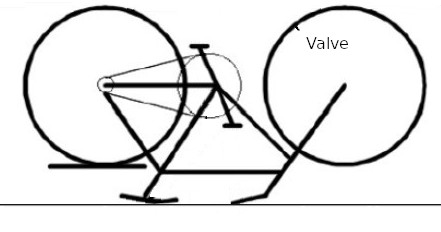
\includegraphics[scale=0.3]{./relativite/valve}
\end{center}

Le référentiel du vélo est ici immobile par rapport au référentiel terrestre.

\end{minipage}
\hfill
\begin{minipage}[c]{.45\linewidth}

Lorsque le cycliste roule en ligne droite et à vitesse constante, le vélo est en {\bf translation rectiligne uniforme} par rapport à la Terre.

%Autrement dit, le référentiel du vélo est en translation rectiligne uniforme par rapport au référentiel terrestre.

\begin{center}
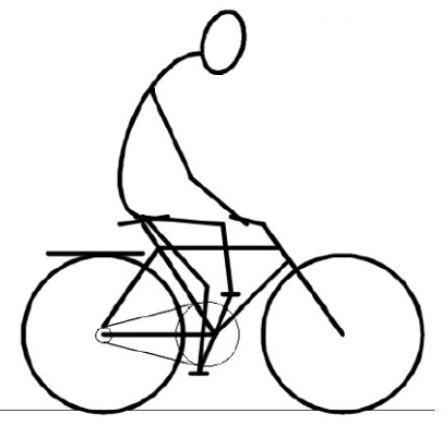
\includegraphics[scale=0.3]{./relativite/velo}
\end{center}

Dans le référentiel terrestre, la trajectoire de la valve n'est plus un cercle.

\end{minipage}


\subsection{L'horloge a lumière}

La technologie fournit des horloges performantes. De façon générale, une horloge fait appel à un phénomène périodique (pendule, oscilateur à ressort, vibration atomique) et à un compteur (cadran à aiguille, électronique).


%%%%%%%%%%%%%%%%%%%%%%%%%%%%%%%%%%%%%%%%%%%%%%%%%%%%%%%%%%%%%%%%%%%%%%%%%%
